\begin{center}
    \textsc{A Few Words About the Proof Complexity}

    \textsc{Speaker: Dmitry Sokolov}
\end{center}

Proof system for a language $L \subseteq \{0, 1\}^*$ is a polynomial-time computable function
$\Pi\colon \{0, 1\}^* \times \{0, 1\}^* \rightarrow \{0, 1\}$ such that: 
\begin{enumerate}
	\item if $x \in L \Leftrightarrow$ there exists $y \in \{0, 1\}^*$ such that $\Pi(x, y) = 1$ (we say
        that $y$ is a proof of $x$);
	\item if $x \notin L \Leftrightarrow$ for all $y \in \{0, 1\}^*, \Pi(x, y) = 0$.
\end{enumerate}


The main task of proof complexity is to quantify the size of the smallest proof required to prove that
some given formula is unsatisfiable. Establishing superpolynomial lower bounds on the sizes in all proof
systems will imply that $\NP \neq \coNP$.

On the one hand in proof complexity, we can give the unconditional lower bounds on the length of proofs at
least in some proof systems (which in itself is valuable and amazing, unlike many other complexity
areas). On the other hand, we have lots of applications of these lower bounds: hard instances for
algorithms, lower bounds on the monotone complexity, etc. In this talk, we start with a brief description
of proof complexity and consider some applications.

\begin{center}
    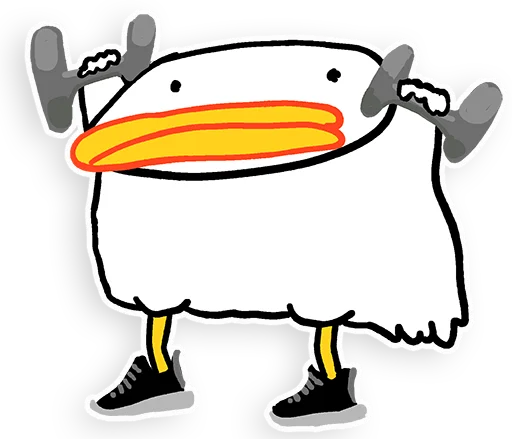
\includegraphics[scale = 0.1]{pics/utia-lift.png}
\end{center}